\PassOptionsToPackage{unicode=true}{hyperref} % options for packages loaded elsewhere
\PassOptionsToPackage{hyphens}{url}
%
\documentclass[10pt,ignorenonframetext,]{beamer}
\setbeamertemplate{caption}[numbered]
\setbeamertemplate{caption label separator}{: }
\setbeamercolor{caption name}{fg=normal text.fg}
\beamertemplatenavigationsymbolsempty
\usepackage{lmodern}
\usepackage{amssymb,amsmath}
\usepackage{ifxetex,ifluatex}
\usepackage{fixltx2e} % provides \textsubscript
\ifnum 0\ifxetex 1\fi\ifluatex 1\fi=0 % if pdftex
  \usepackage[T1]{fontenc}
  \usepackage[utf8]{inputenc}
  \usepackage{textcomp} % provides euro and other symbols
\else % if luatex or xelatex
  \usepackage{unicode-math}
  \defaultfontfeatures{Ligatures=TeX,Scale=MatchLowercase}
\fi
\usetheme[]{CambridgeUS}
\usecolortheme{dove}
\usefonttheme{structurebold}
% use upquote if available, for straight quotes in verbatim environments
\IfFileExists{upquote.sty}{\usepackage{upquote}}{}
% use microtype if available
\IfFileExists{microtype.sty}{%
\usepackage[]{microtype}
\UseMicrotypeSet[protrusion]{basicmath} % disable protrusion for tt fonts
}{}
\IfFileExists{parskip.sty}{%
\usepackage{parskip}
}{% else
\setlength{\parindent}{0pt}
\setlength{\parskip}{6pt plus 2pt minus 1pt}
}
\usepackage{hyperref}
\hypersetup{
            pdftitle={Predicting crime rates using taxi rides in NYC},
            pdfborder={0 0 0},
            breaklinks=true}
\urlstyle{same}  % don't use monospace font for urls
\newif\ifbibliography
% Prevent slide breaks in the middle of a paragraph:
\widowpenalties 1 10000
\raggedbottom
\AtBeginPart{
  \let\insertpartnumber\relax
  \let\partname\relax
  \frame{\partpage}
}
\AtBeginSection{
  \ifbibliography
  \else
    \let\insertsectionnumber\relax
    \let\sectionname\relax
    \frame{\sectionpage}
  \fi
}
\AtBeginSubsection{
  \let\insertsubsectionnumber\relax
  \let\subsectionname\relax
  \frame{\subsectionpage}
}
\setlength{\emergencystretch}{3em}  % prevent overfull lines
\providecommand{\tightlist}{%
  \setlength{\itemsep}{0pt}\setlength{\parskip}{0pt}}
\setcounter{secnumdepth}{0}

% set default figure placement to htbp
\makeatletter
\def\fps@figure{htbp}
\makeatother

\author{Carlos Petricioli \and
    Varsha Muralidharan   \and
    Valerie Angulo  }

\institute[New York University]{ New York University \\ \{cpa253,vm1370,vaa238\}@nyu.edu }

\setbeamerfont{headline}{size=\fontsize{8}{1}\selectfont}
\setbeamertemplate{headline}
{
  \leavevmode%
  \hbox{%
  \begin{beamercolorbox}[wd=1\paperwidth,ht=2.3ex,dp=1.5ex,right]{section in head/foot}%
    \usebeamerfont{section in head/foot}\insertsectionhead\hspace*{1ex}
  \end{beamercolorbox}%
  % \begin{beamercolorbox}[wd=0\paperwidth,ht=2.65ex,dp=1.5ex,right]{subsection in head/foot}%
  %   \usebeamerfont{subsection in head/foot}\hspace*{2ex}\insertsubsectionhead
  % \end{beamercolorbox}
  }%
  \vskip0pt%
}


% \setbeamertemplate{navigation symbols}{}
% \setbeamertemplate{footline}[page number]
\setbeamertemplate{footline}
{
  \leavevmode%
  \hbox{%
      \begin{beamercolorbox}[wd=1\paperwidth,ht=2.25ex,dp=1ex,right]{author in head/foot}%
          \usebeamerfont{author in head/foot}
          \insertframenumber{} of  \inserttotalframenumber\hspace*{2ex} 
      \end{beamercolorbox}}%
      \vskip0pt%
}

% Set Color ==============================
% Custom colors
\usepackage{xcolor}

%\definecolor{gold}{HTML}{FDD017}
\definecolor{gold}{HTML}{fdde5c}
% \definecolor{deep sky blue}{HTML}{3BB9FF}
% \definecolor{light sky blue}{HTML}{82CAFA}

\makeatletter
\definecolor{mybackground}{HTML}{fef5d0}
\definecolor{myforeground}{HTML}{0000A0}

\setbeamercolor{normal text}{fg=black,bg=white}
\setbeamercolor{alerted text}{fg=red}
\setbeamercolor{example text}{fg=black}

\setbeamercolor{block title}{bg=mybackground,fg=black}


\setbeamercolor{background canvas}{fg=myforeground, bg=white}
\setbeamercolor{background}{fg=myforeground, bg=mybackground}

\setbeamercolor{palette primary}{fg=black, bg=gray!30!white}
\setbeamercolor{palette secondary}{fg=black, bg=gray!20!white}
\setbeamercolor{palette tertiary}{fg=black, bg=gold}
\makeatother

\title{Predicting crime rates using taxi rides in NYC}
\date{12/15/2017}

\begin{document}
\frame{\titlepage}

\begin{frame}{%
\protect\hypertarget{big-data-analytics-symposium---fall-2017}{%
Big Data Analytics Symposium - Fall 2017}}

\begin{block}{Analytics Project}

Predicting crime rates using taxi rides in NYC

\end{block}

\begin{block}{Team}

\begin{itemize}
\item
  Carlos Petricioli (cpa253)
\item
  Varsha Muralidharan (vm1370)
\item
  Valerie Angulo (vaa238)
\end{itemize}

\end{block}

\begin{block}{Abstract}

\begin{itemize}
\tightlist
\item
  We study crime rates and its relationship on how people use of taxis
  in New York City.
\item
  Our hypothesis is that people are less likely to walk in areas
  subjectively deemed more dangerous and will instead opt to use more
  reliable and immediate transportation such as designated taxis.
\item
  WE FOUND THAT \_\_\_\_.
\end{itemize}

\end{block}

\end{frame}

\hypertarget{predicting-crime-rates-using-taxi-rides-in-nyc}{%
\section{Predicting crime rates using taxi rides in
NYC}\label{predicting-crime-rates-using-taxi-rides-in-nyc}}

\begin{frame}{%
\protect\hypertarget{motivation}{%
Motivation}}

\begin{block}{Typical user of this application}

The scientific community, the citizens and demographics themselves.

\end{block}

\begin{block}{Insight that we’ll get}

The objective is to get a better sense of the way that crime relates to
the use of taxis in NYC.

\end{block}

\end{frame}

\begin{frame}{%
\protect\hypertarget{goodness}{%
Goodness}}

\begin{block}{cleaning data}

we made sure that –

\end{block}

\begin{block}{model testing}

we made sure that –

\end{block}

\end{frame}

\begin{frame}{%
\protect\hypertarget{data-sources}{%
Data Sources}}

\begin{block}{Taxi rides data form TLC
\href{http://www.nyc.gov/html/tlc/html/about/trip_record_data.shtml}{(\emph{Link})}}

\begin{itemize}
\item
  It covers years from 2009 to June 2017.
\item
  The yellow taxi trip records include:

  \begin{itemize}
  \tightlist
  \item
    pick-up and drop-off dates/times,
  \item
    pick-up and drop-off locations,
  \item
    trip distance,
  \item
    itemized fares,
  \item
    rate types,
  \item
    payment type,
  \item
    passenger counts.
  \end{itemize}
\end{itemize}

\end{block}

\end{frame}

\begin{frame}

\begin{block}{NYPD Complaint Data
\href{https://data.cityofnewyork.us/Public-Safety/NYPD-Complaint-Data-Historic/qgea-i56i}{(\emph{Link
1,}}
\href{https://data.cityofnewyork.us/Public-Safety/NYPD-Complaint-Data-Current-YTD/5uac-w243}{\emph{Link
2)}}}

\begin{itemize}
\tightlist
\item
  This dataset includes all valid felony, misdemeanor, and violation
  crimes reported to the New York City Police Department (NYPD) from
  2006 to year to date data.
\end{itemize}

\end{block}

\begin{block}{NOAA Weather stations data
\href{https://www.ncdc.noaa.gov/isd}{\emph{(Link)}}}

The \emph{Integrated Surface Database (ISD)} consists of global hourly
ansynoptic observations compiled from numerous sources into a single
common ASCII format and common data model.

\begin{itemize}
\item
  ISD’s complete history of hour-by-hour readings for one user-specified
  weather stations
\item
  We selected:

  \begin{itemize}
  \tightlist
  \item
    Central Park
  \item
    JFK
  \item
    Laguardia
  \end{itemize}
\end{itemize}

\end{block}

\end{frame}

\begin{frame}{%
\protect\hypertarget{design-diagram}{%
Design Diagram}}

\begin{center}
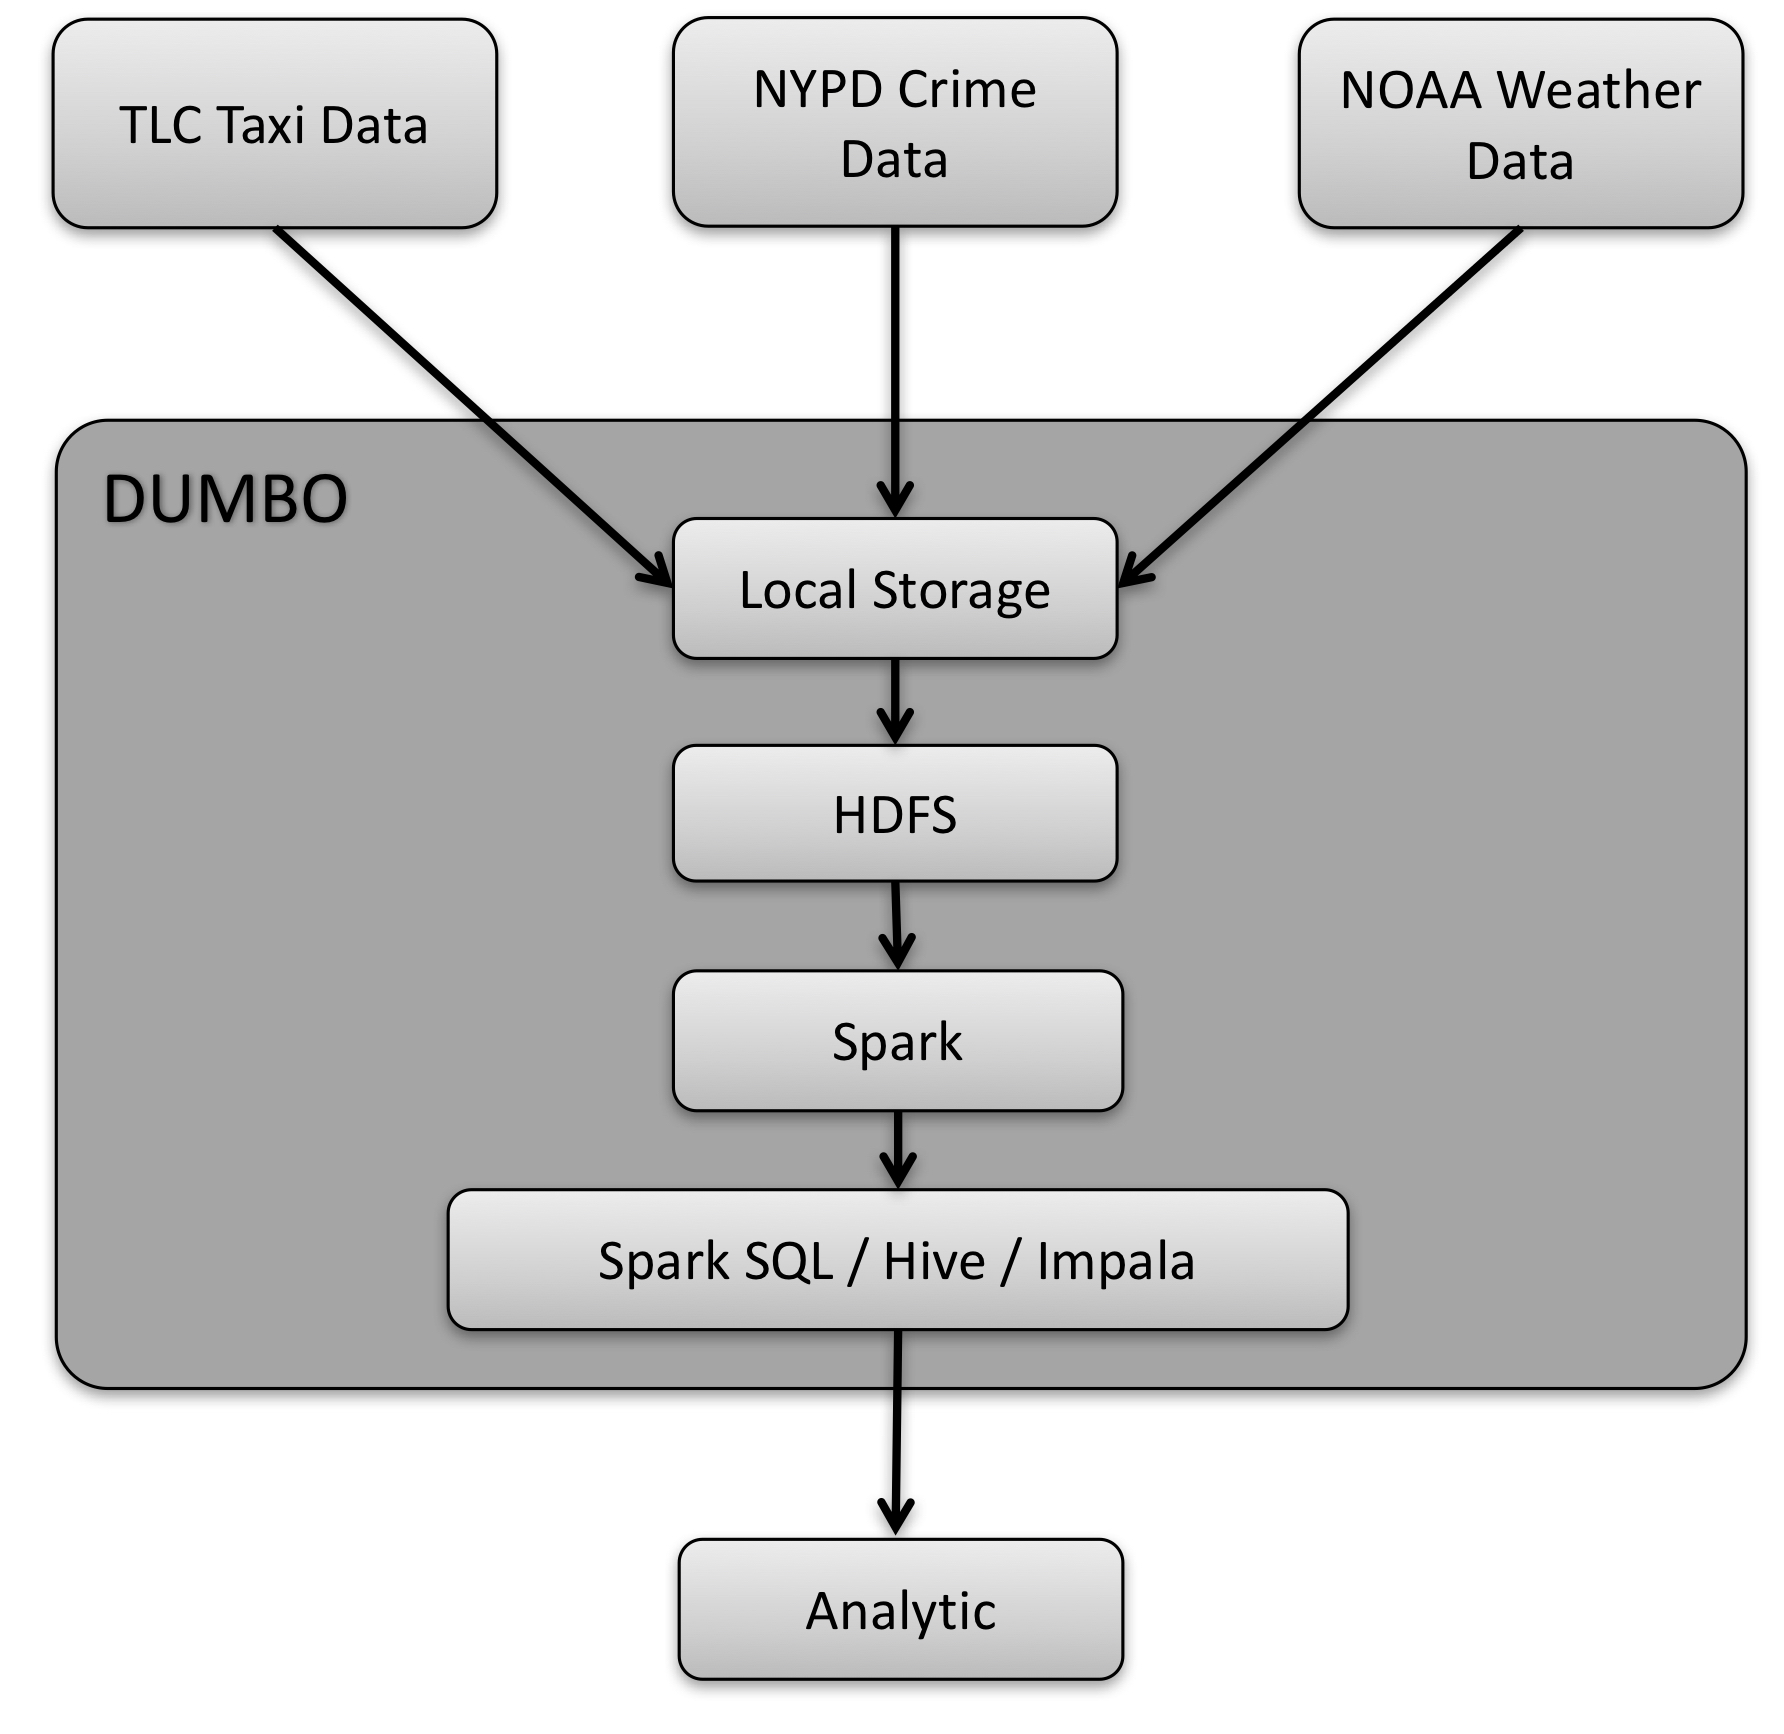
\includegraphics[height=.6\textheight]{img/DesignFlowDiagram.jpg}
\end{center}

\begin{block}{Platform:}

\begin{itemize}
\tightlist
\item
  NYU HPC cluster (Dumbo)
\end{itemize}

\end{block}

\end{frame}

\begin{frame}{%
\protect\hypertarget{results}{%
Results}}

\begin{enumerate}
[1.]
\item
  Result 1
\item
  Result 2
\item
  Result 3
\end{enumerate}

\end{frame}

\begin{frame}{%
\protect\hypertarget{obstacles}{%
Obstacles}}

\begin{enumerate}
[1.]
\item
  Obstacle 1
\item
  Obstacle 2
\end{enumerate}

\end{frame}

\begin{frame}{%
\protect\hypertarget{summary}{%
Summary}}

Brief wrap-up!

\end{frame}

\begin{frame}{%
\protect\hypertarget{acknowledgements}{%
Acknowledgements}}

We thank the people from HPC support at NYU. Specially Santhosh Konda
\href{mailto:hpc@nyu.edu}{\nolinkurl{hpc@nyu.edu}} for being reachable
with very short response time.

\end{frame}

\begin{frame}{%
\protect\hypertarget{references}{%
References}}

\begin{thebibliography}{1}

\bibitem{Bendler14}
J.~Bendler, T.~Brandt, S.~Wagner, and D.~Neumann.
\newblock Investigating crime-to-twitter relationships in urban environments -
  facilitating a virtual neighborhood watch.
\newblock In M.~Avital, J.~M. Leimeister, and U.~Schultze, editors, {\em ECIS},
  2014.

\bibitem{fbiUniformCrime}
{Federal Bureau of Investigation, Uniform Crime Reporting}.
\newblock {Offenses Known to Law Enforcement by State by City}.
\newblock 2016.

\bibitem{Traunmueller14}
M.~Traunmueller, G.~Quattrone, and L.~Capra.
\newblock {\em Mining Mobile Phone Data to Investigate Urban Crime Theories at
  Scale}, pages 396--411.
\newblock Springer International Publishing, Cham, 2014.
\end{thebibliography}

\end{frame}

\begin{frame}

\begin{thebibliography}{1}
\bibitem{Wang16}
H.~Wang, D.~Kifer, C.~Graif, and Z.~Li.
\newblock Crime rate inference with big data.
\newblock In {\em Proceedings of the 22Nd ACM SIGKDD International Conference
  on Knowledge Discovery and Data Mining}, KDD '16, pages 635--644, New York,
  NY, USA, 2016. ACM.

\end{thebibliography}

\end{frame}

\hypertarget{thank-you}{%
\section{Thank you!}\label{thank-you}}

\end{document}
